\documentclass{article}
\usepackage[utf8]{inputenc}
\usepackage{amsmath,amssymb,amsfonts,amsthm,graphicx,enumitem,algorithm,algorithmic}
\usepackage[parfill]{parskip}
\usepackage{color}
\usepackage{float}
\DeclareMathOperator*{\argmin}{arg\,min}
\DeclareMathOperator*{\argmax}{arg\,max}
\usepackage[top=1in,bottom=1in,left=1.4in,right=1.4in]{geometry}

\title{ \vspace{-5mm}
        "PDE methods for option pricing" study notes}         % <-- Edit Homework Number
\author{\Large{Jian Wang}\\      % <-- Edit Name
\\
FSU ID: jw09r}        % <-- Edit Andrew Id

\begin{document}
\maketitle
\section*{Chapter 1}
20150107 Monday
\large{
What is an option?\\

\textbf{Problem 1:} Stock today \$100, in one year \$110\\
\hspace*{2.5cm} $\Longrightarrow$ 10\% profit and at risk \$100, which is 100\% loss. \\

\textbf{Problem 2:} Leverage \$10 borrow \$90 = \$100\\
\hspace*{2.5cm} \underline{in a year \hspace*{3.1cm}  \$110}\\
\hspace*{6.5cm} \$20 Profit \\
\hspace*{5cm} $\Longrightarrow$ 100\%(20-10/10),at risk \$100({\color{red}{10+investment}})

\textbf{Problem 3:} Call option: right to buy at an agreed on price in one year.\\

$S_{today}=\$100$\\

$S_{1 year}=\$110$\\

Want 20\% profit\\

Buy option to purchase the stock at price \$92 \\

In 1 year: we can buy the stock at price \$92(according to the right of call option), and can sell the stock to the market at price \$110. the profit is \$18.\\
cost is the value of the option.$\rightarrow$ How do we compute?\\
at risk $\mathcal{V}$=option price\\

\underline{A two state example} \\
\\
Assume S(0)=\$100\\
In one year
\begin{equation*}
S(1)=\left\{
\begin{tabular}{l}
\$110  \\
\$90
\end{tabular}
\right.
\end{equation*}

buying price \$92\\
\begin{equation*}
\begin{tabular}{c|rl}
 Today&T&=1\\
 \hline
 s=100&s=\$110&s=\$90  \\
 $\mathcal{V}$=?&\$18&0
\end{tabular}
\end{equation*}
Here 0 is payoff\\
Set up portfolio : \\
Buy n share stock and sell one call option:\\
\begin{equation*}
P(T)=n\cdot110 - 18 \qquad\qquad P(T)=n\cdot90 - 0
\end{equation*}
risk free: \\
\begin{equation*}
\begin{aligned}
n\cdot110 - 18=90\cdot n\\
solve:\quad \fbox{n=\$0.9}
\end{aligned}
\end{equation*}

Value of portfolio, $P(T)=\$81$\\
Today it is worth, need present value of \$81\\
If we put into bank \\
\begin{equation*}
\begin{aligned}
\frac{dp}{dt}=rp\\
P(T)=p(0)e^{rt}\\
P(0)=e^{-rt}P(T)
\end{aligned}
\end{equation*}
Here r is the risk free rate and the $e{-rt}$ is the discount factor., if $r=0.05, year 1, p(0)=e^{-0.05}\times \$81 =\$77$(portfolio value today).\\

Today:
\begin{equation*}
\left\{
\begin{aligned}
100\times0.9-\mathcal{V}=\$77  \\
\mathcal{V}=\$13
\end{aligned}
\right.
\end{equation*}

\clearpage
20150109  Wednesday option pricing
\begin{table}[!htp]
\newcommand{\tabincell}[2]{\begin{tabular}{@{}#1@{}}#2\end{tabular}}
  \centering
\begin{tabular}{ll}
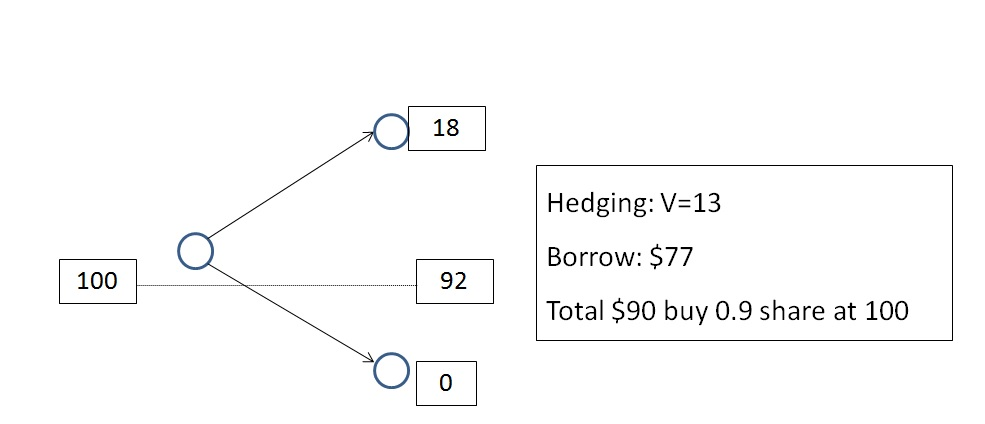
\includegraphics[height=2in,width=3.5in]{hedging.jpg}&\tabincell{c}{hedging $\mathcal{V}$=\$13 \\\\ Borrow \$ 47 \\\\ Total \$90 buy 0.9 share at \$ 100}
\end{tabular}
\end{table}
\\
In a year:\\
\begin{table}[!htp]
\newcommand{\tabincell}[2]{\begin{tabular}{@{}#1@{}}#2\end{tabular}}
  \centering
\begin{tabular}{ll}
(1) s=\$110 &\tabincell{c}{so owe (0.9)$\times$ 110=\$99\\owe 18 to "BOB" lending \$81\\owe 77$\times exp^{0.05}=\$81$}\\
\\
(2)s=\$90& we have (0.9)$\times$90=\$81 pay bank
\end{tabular}
\end{table}
\\
Stocks don't work like this, they have random component, If there wasn't we expect.\\

$\frac{dS}{S}= \mu dt$, here $\mu$ is the drift rate.\\

know at t, $ S = S_0 e^{\mu t}$\\

Otherwise add random component\\

$\frac{dS}{S}=\mu dt + \sigma dZ$\\

$dZ = \phi \sqrt{dt}$: $\phi: normal distribution$ with mean 0 and variance 1\\

What is S(t)? \\

Def expectation:\\
$E(Y)=E[f(\phi)]$: Here f($\phi$) is a random variable\\
$=\int_{\Omega}f(\phi)P(\phi)d\phi$ : Here $P(\phi)$ is the probability density function\\
e.g:
\begin{flalign*}
&P(\phi)=\frac{1}{\sqrt{s\pi}}e^{-1/2\phi^2}&\\
&E[1]=\frac{1}{\sqrt{2 \pi}}\int_{-\infty}^{\infty}e^{-1/2\phi^2}d\phi=1&\\
&E[\phi]=\frac{1}{\sqrt{2 \pi}}\int_{-\infty}^{\infty}\phi e^{-1/2\phi^2}d\phi=0&\\
&E[\phi^2]=\frac{1}{\sqrt{2 \pi}}\int_{-\infty}^{\infty}\phi^2 e^{-1/2\phi^2}d\phi=1&\\
&E[\frac{dS}{S}]=E[\mu dt+\sigma dZ]&\\
&=\mu E[dt]+\sigma E[dZ]&\\
&=\mu dtE[1](=1, coz\quad no\quad variation)+\sigma \sqrt{dt}E[d\phi]&(=0,coz\quad Gaussian\quad disstribution)\\
&=\mu dt& \\
&Var[Y]=E[Y^2]-E^2[Y]&\\
&Var[\phi]=E[\phi^2]=E[\phi^2]-E^2[\phi]=1&\\
&Var[\frac{dS}{S}]=E[(\frac{dS}{S})^2]-E^2[\frac{ds}{s}]&\\
&since:\frac{dS}{S}=\mu dt+\sigma \phi\sqrt{dt}&\\
&E[(\frac{dS}{S})^2]=E[(\mu dt +\sigma \sqrt{dt}\phi)^2]&\\
&=(\mu dt)^2+2\mu \sigma dt E[dZ]+\sigma^2E[(dZ)^2]-(\mu dt)^2&\\
&=\sigma^2 dt&
\end{flalign*}
$\sigma \rightarrow$ volatility standard deviation\\

Lemma($it\hat{o}$) suppose $G=G(s,t)$ where $\frac{dS}{S}=\mu dt + \sigma dZ$\\

then: $dG=(\mu S\frac{dG}{dS}+ \frac{\sigma^2 S^2}{2}\frac{\partial^2 G}{\partial S^2}+\frac{\partial G}{\partial t})dt+\sigma S \frac{\partial G}{\partial S}d\mathcal{Z}$\\

To find $S(t)$, let $G(s)=log(s), G_s=\frac{1}{S}, G_t=0, G_{SS}=-\frac{1}{S^2}$\\

$dG=G_SS\sigma d\mathcal{Z}+(\mu S G_S+\frac{\sigma^2 S^2}{2}G_{SS}+G_t)dt$\\
Substitution for partial derivatives,\\
$=\sigma d{\mathcal{Z}}+\mu dt -\frac{\sigma^2}{2}dt$\\

$dG=\sigma d\mathcal{Z}+(\mu-\frac{\sigma^2}{2})dt$\\

$\int_{0}^{t}dG=\sigma \int_{0}^{t}d\mathcal{Z}+(c)\int_{0}^{t}dt$

$G(t)-G(0)=\sigma (\mathcal{Z}(t)-\mathcal{Z}(0))+(\mu-\frac{\sigma^2}{2})t$\\

$G=log(S)$\\

$log(S)-log(S_0)=\sigma (\mathcal{Z}(t)-\mathcal{Z}(0))+(\mu-\frac{\sigma^2}{2})t$\\

$\Longrightarrow$ \fbox{$S=s_0 e^{\sigma(\mathcal{Z}(t)-\mathcal{Z}(0))+(\mu -\frac{\sigma^2}{2})t}$}

Black-Scholes Equation\\
Assume (1)the stock price follows a geometric brownian motion\\
(2)Risk free rate is $r$ = constant and also $\sigma$ = constant\\
(3) No arbitrage ("All risk-free portfolio grow at risk free rate")\\
Set up portfolio with one option and a share of stocks (borrowed)\\
\begin{flalign*}
&P=V - \alpha S&\\
&dP=dV-\alpha ds&\\
&dp= dV-\alpha ds=dV-\alpha (\mu dt +\sigma d\mathcal{Z})S&\\
&dV(s)=(\mu s V_s+\frac{\sigma^2 s^2}{2}V_{SS}+V_t)dt+\sigma S V_s d\mathcal{Z}&\\
\end{flalign*}
$\Rightarrow$ $dP=\sigma S(V_s-\alpha)d\mathcal{Z}+(\mu S V_s + \frac{\sigma^2S^2}{2}V_{SS}+V_t-\alpha \mu_s)dt$\\
If we choose $\alpha = V_s$, $dP$ doesn't depend on $d\mathcal{Z}$\\
So: $dP=(\mu s V_s- \alpha(=V_s) \mu_s +\frac{\sigma^2S^2}{2}V_{SS}+V_t)dt$\\
$dP=(\frac{\sigma^2S^2}{2}V_{SS}+V_t)dt=rPdt$\\
with: $P=V-V_{S}S \Rightarrow V_t + \frac{\sigma^2 S^2}{2}V_{SS}+rSV_s-rV=0(*)$\\

\newpage
20150112 Monday option pricing \\
Hedging: \\
(1)Sell option of value V computed by * \\

(2) Buy $SV_s-V$ from bank \\

(3) Buy $V_s$ shares of stocks($SV_s$)\\

always keep $V_s$ shares $\Leftrightarrow$ Dynamic hedge \\

$\Delta =V_s$\\

Greeks:\\

\begin{tabular}{ccc}
Name&Symbol&Def\\
Delta&$\Delta$&$V_s$  \\
Gamma&$\Gamma$&$V_{ss}$\\
Vega&$\nu$&$V_{\sigma}$\\
Rho&$\rho$&$V_{r}$\\
Theta&$\Theta$&$V_t
$\\
\end{tabular}

Knowing V we can compute \\
eg. $\Delta$ and $\Gamma$ by finite differences ${V_j}_{j=0}^N$\\
$\Delta_j\approx \delta_x^0V_j=\frac{V_{j+1}-V_{j-1}}{2\Delta S}$\\
$\Gamma_j \approx \delta_x^{+}\delta_x^{-}V_j=\frac{V_{j+1}-2V_j+V_{j-1}}{\Delta S^2}$

To get $\rho$ or $\nu$, use two values $r\pm \Delta r$\\
Gives $\frac{V_j(r+\Delta r)-V_j(r-\Delta r)}{2\Delta r}\approx \rho_j$\\
But the Greeks also satisfy advection-diffusion equations:\\
eg:find equation for $\Delta$\\
\begin{flalign*}
&\frac{\partial}{\partial S}(V_t+\frac{\sigma^2S^2}{2}V_{SS}+rSV_S-rV)=0(remark: BS.equation)&\\
&(V_s)_t+\sigma^2SV_{SS}+\frac{\sigma^2S^2}{2}V_{SSS}+rV_s+rSV_{SS}-rV_S=0&\\
&\Delta_t+\sigma^2SV_{SS}+\frac{\sigma^2S^2}{2}V_{SSS}+r\Delta+rS\Delta_S-r\Delta=0&\\
&\Delta_t+\frac{\sigma^2S^2}{2}\Delta_{SS}+(\sigma^2+r)S\Delta_S=0&\\
\end{flalign*}
Similar for $\Gamma$\\

For $\rho$:\\

\begin{align*}
&\frac{\partial}{\partial r}(V_t+\frac{\sigma^2S^2}{2}V_{SS}+rSV_S-rV)=0\\
&(V_r)_t+\frac{\sigma^2S^2}{2}(V_r)_{SS}+SV_S+SV_S+rs(V_r)_S
-V-rV_r=0\\
\end{align*}

\begin{equation*}
\begin{aligned}
\begin{cases}
&\rho_t+\frac{\sigma^2S^2}{2}(\rho)_{SS}+SV_S+rs(\rho)_S-r\rho+SV_S-V=0\\
&V_t+\frac{\sigma^2S^2}{2}V_{SS}+rSV_S-rV=0\\
\end{cases}
\end{aligned}
\end{equation*}
$\left[
\begin{tabular}{l}
$\rho$  \\
$V$
\end{tabular}
\right]_t=\vec{q}_t$
\begin{flalign*}
&\vec{q}_{SS}|_j\approx \delta_{S}^{+}\delta_{S}^{-}\vec{q}_j&\\
&V_S|_j\approx \delta_S^0V|_j&\\
\end{flalign*}

Need BC's and final conditions\\

(B-S equation is backward diffusion equation)\\

forward in $\tau=T-t$\\
so we change $\frac{\partial}{\partial t}=\frac{\partial}{\partial t}\frac{\tau}{\partial t}=-\frac{\partial }{\partial \tau}$\\

$V_\tau - \frac{\sigma^2 S^2}{2}V_{SS}-rSV_S+rV=0$\\

The I.C. tell us the type of option +exercise rights\\

European options: Can only exercise at $t=T$\\

American options : Can exercise any time between $t=[0,T]$\\

Two vanilla Europe options \\
(1)European call \\
Right to buy S at $t=T$ (expiry at T ), but not obligation \\
$V(\tau =0)=pay off =max (S-k,0)$(Here S is underlying and K is the exercise price)\\
$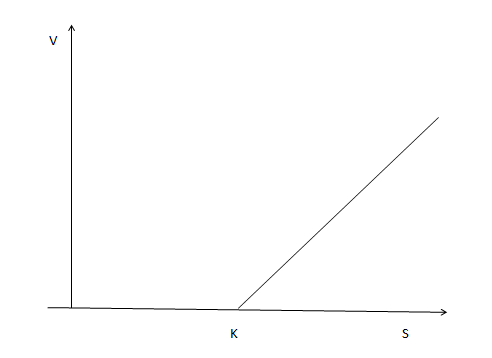
\includegraphics[height=2in,width=3.5in]{callpayoff.png}$\\

Put: right to sell S at price K at time t. payoff =$max(K-S,0)$,payoff $\notin C^2$
$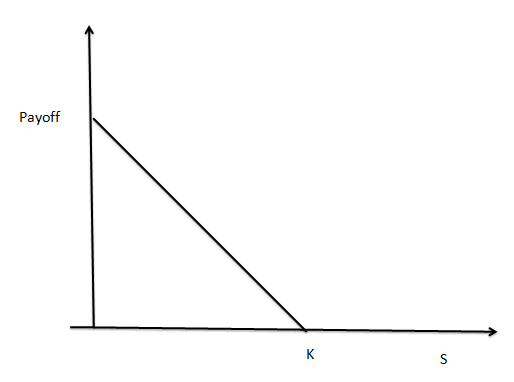
\includegraphics[height=2in,width=3.5in]{putpayoff.png}$\\

Note for $\Delta$:\\
$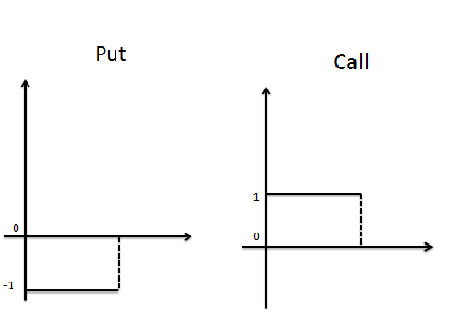
\includegraphics[height=2.5in,width=4in]{deltaputcall.png}$\\

For Gap option:\\

\begin{table}[!htp]
$V_{call}(t=T)=\left\{
\begin{tabular}{ll}
$S-K$&$K^{'} <S$\\
0&otherwise
\end{tabular}
\right.$
\end{table}
$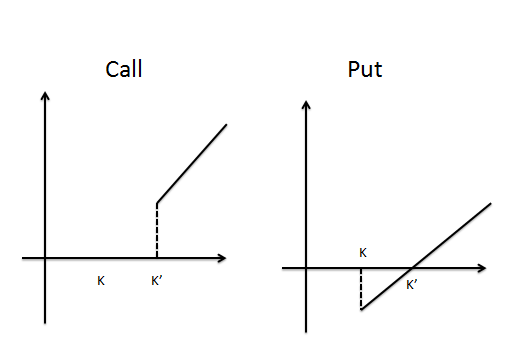
\includegraphics[height=2.5in,width=4in]{gapoptions.png}$\\
For vanilla options:\\
$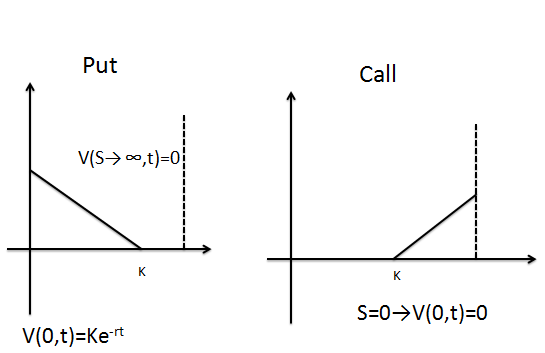
\includegraphics[height=2.5in,width=4in]{vanillaoptions.png}$

\newpage
20150206 Friday option pricing\\
\\
$w_t+\frac{\sigma^2}{2}W_{xx}+(r-\frac{\sigma^2}{2})$\\
\\
Here $W_t$ is forward time, given final condition.\\
\\
$\delta_t^{-}W_j^{n+1}+\frac{\sigma^2}{2}\delta_x^{+}\delta_x^{-}W_j^{n+1}+(r-\frac{\sigma^2}{2})\delta_x^0=0$\\
\\
$n=N_t,...,0$\\
\\
write out and gather terms.\\
\\
$W_j^n=(\frac{\sigma^2}{2}\frac{\Delta t}{\Delta x^2}-(r-\frac{\sigma^2}{2})\frac{\Delta t}{2\Delta x})W_{j-1}^{n+1}+(1-\frac{\sigma^2 \Delta t}{\Delta x^2})W_j^{n+1}+(\frac{\sigma^2}{2}\frac{\Delta t}{\Delta x^2}+(r-\frac{\sigma^2}{2})\frac{\Delta t}{2\Delta x})W_{j+1}^{n+1}$\\
\\
Binomial: $V_j^{n}=e^{-r\Delta t}(P V_{j+1}^{n+1}+(1-p)V_j^{n+1})$\\
\\
we choose $\Delta x$ so that :\\
\\
\begin{center}
$\frac{\sigma^2}{2}\frac{\Delta t}{\Delta x^2}-(r-\frac{\sigma^2}{2})\frac{\Delta t}{2\Delta x}=0$
\end{center}
\begin{center}
\begin{table}[!htp]
\centering
\begin{tabular}{ll}
\fbox{$\Delta x=\frac{\sigma^2}{r-\frac{\sigma^2}{2}}$}&$\frac{\sigma^2}{2}\frac{\Delta t}{\Delta x^2}\leq \frac{1}{2}$
\end{tabular}
\end{table}
\end{center}

Then: $W_j^{n}=PW_{j+1}^{n+1}+(1-p)W_j^{n+1}$\\
$P=\frac{\Delta t(r-\frac{\sigma^2}{2})}{\sigma^2}$\\
$V_j^{n+1}=e^{rt_{n+1}}W_j^{n+1}$\\
$V_j^{n}=e^{rt_{n}}W_j^{n}$\\
so: $V_j^n=e^{-r\Delta t}\{PV_{j+1}^{n+1}+(1-p)V_j^{n+1}\}$\\
$\rightarrow$ For Binomial tree:\\
(1) $1^{st}$ order in time (not accurate, however, manager like it since easy)\\
(2)stability limit for $\Delta t$\\
$\color{red}{\frac{2^P}{2^p-1},\frac{2}{1},...,0}$\\
$R_{Exact}\approx R_{\Delta x} +C\Delta x^P$\\
$R_{Exact}\approx R_{\frac{\Delta x}{2}} +C(\frac{\Delta x^P}{2})$\\
$\Rightarrow 0\approx (R_{\Delta x}-R_{\frac{\Delta x}{2}})+C\Delta x^P(1-\frac{1}{2^P})$(remark:$C\Delta x^P$ is Error, $C\Delta x^P=E\Delta_x$)
$\Rightarrow E_{\Delta x}\approx \frac{2^P}{2^p-1}(R_{\frac{\Delta x}{2}}-R_{\Delta x})$\\
$w_t+\frac{\sigma^2}{2}W_{xx}+(r-\frac{\sigma^2}{2})$\\
$X=log(S)
$\\
$S\in (0,\infty)$\\
$x\in (-\infty,\infty)$\\

\begin{table}[!htp]
\begin{tabular}{ll}
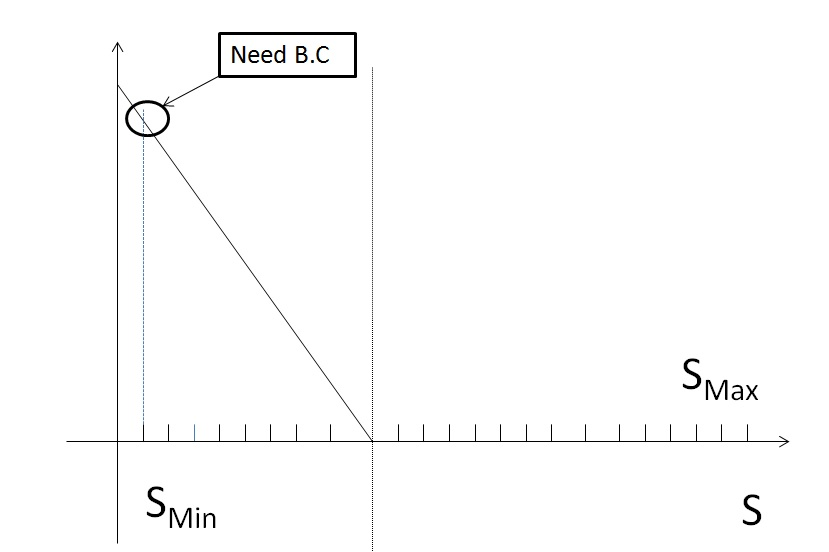
\includegraphics[height=2in,width=3in]{stock1.jpg}&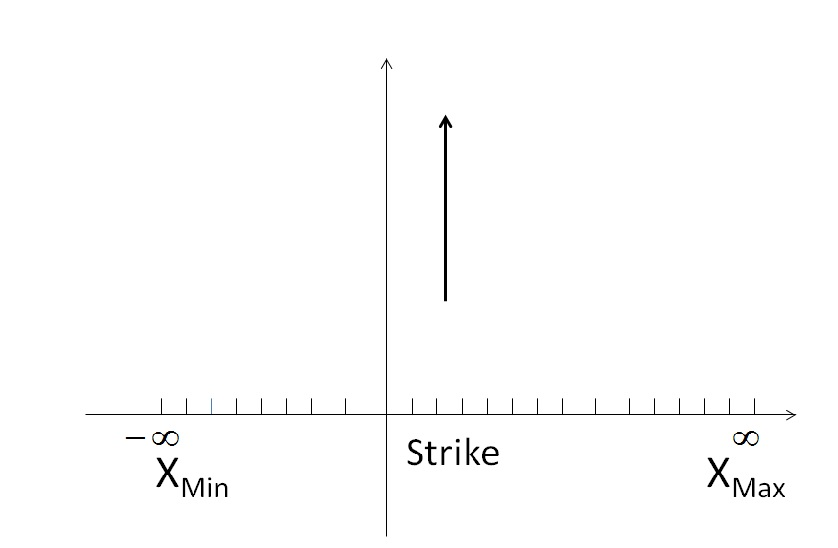
\includegraphics[height=2in,width=3in]{stock2.jpg}
\end{tabular}
\end{table}
Next Time European options with Jump Diffusion Diffusion:\\
\\
$V_t+\frac{\sigma^2S^2}{2}V_{SS}+(r-\kappa \lambda)SV_s-(r+\lambda)V+\int_{0}^{\infty}V(JS,t)g(J)dJ)=0$\\

\newpage 
20150213 Friday option pricing \\

$\widetilde{I_j}=\sum_{l=-N/2}^{N/2-1} V_{j-l}\tilde{\tilde{g_l}}$\\

}
\end{document} 